\Chapter {Tesztelés a gyakorlatban}
Minden teszt esethez tartoznak különböző információk, amik változnak a cég által használt rendszertől függően. Lehetséges, hogy egy teszt esetet létre tud hozni a kreálója, minden mellék információ megadása nélkül, de általában van néhány alap feltétel is amiket az én programom keretében a \aref{fig:template} kép mutatja be.\\

\label {tab:template}
\label {tab:testcase}
\label {tab:successcase}

\begin{figure} [h]
	\centering
	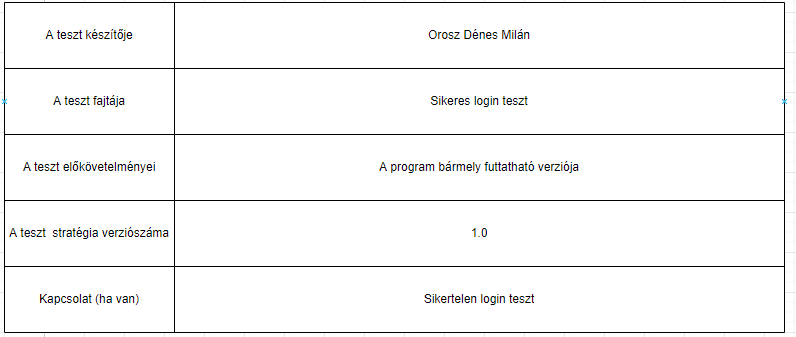
\includegraphics[scale=0.86]{images/test_case_template.png}
	\caption{A teszt esethez tartozó információk.}
	\label{fig:template}
\end{figure}
Minden teszt eset 3 vagy 4 oszlopból áll. Az első oszlopban a lépés sorszáma, a másodikban  maga a lépés van megfogalmazva, a harmadik és negyedik oszlop pedig az elvárt eredményt, illetve a lépéshez tartozó bemenetet tartalmazzák, viszont előfordulhat, hogy a bemeneteket egy másik táblázatban tárolják. Példát erre a \aref{fig:testcase} mutatja be.\\

\begin{figure}[h]
	\centering
	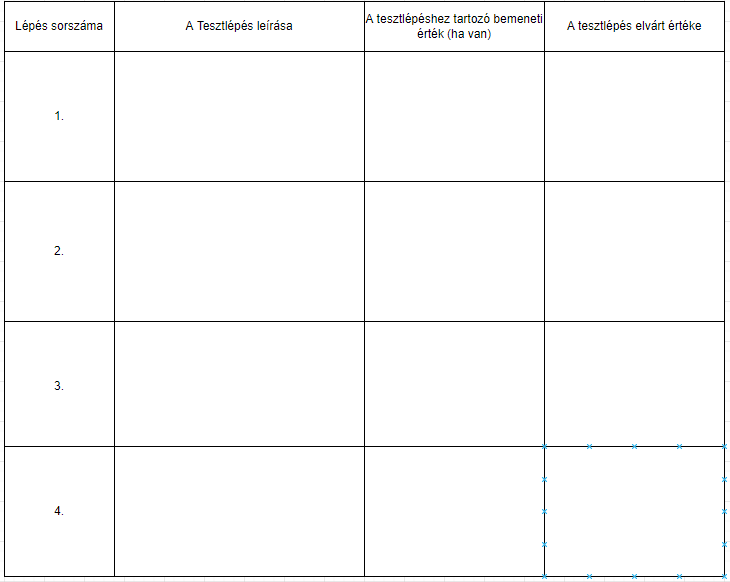
\includegraphics[scale=0.86]{images/test_case.png}
	\caption{Egy teszt eset teszt lépések nélkül}
	\label{fig:testcase}
\end{figure}



\begin{figure}
	\centering
	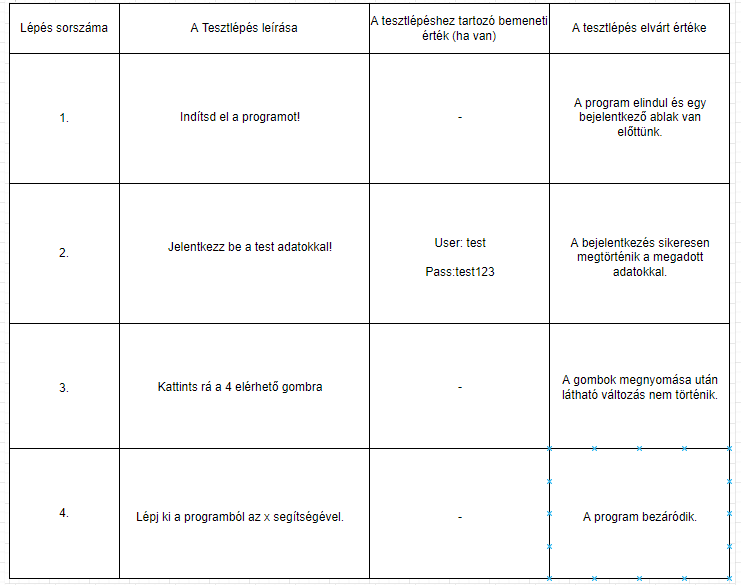
\includegraphics[scale=0.86]{images/success_login_test_case.png}
	\caption{A programhoz tartozó sikeres bejelentkezés teszt esete}
	\label{fig:successcase}
\end{figure}

A \aref{fig:successcase} képen látható, az én programomhoz tartozó bejelentkezést tesztelő teszt esetnek a lépéssorozata és a hozzá tartozó bemenetek és az elvárt eredmények.

\Chapter{Megvalósítás}

Ez a fejezet mutatja be a megvalósítás lépéseit.
Itt lehet az esetlegesen előforduló technikai nehézségeket említeni.
Be lehet már mutatni a program elkészült részeit.

Meg lehet mutatni az elkészített programkód érdekesebb részeit.
(Az érdekesebb részek bemutatására kellene szorítkozni.
Többségében a szöveges leírásnak kellene benne lennie.
Abból lehet kiindulni, hogy a forráskód a dolgozathoz elérhető, azt nem kell magába a dolgozatba bemásolni, elegendő csak behivatkozni.)

A dolgozatban szereplő forráskódrészletekhez külön vannak programnyelvenként stílusok.
Python esetében például így néz ki egy formázott kódrészlet.
\begin{python}
import sys

if __name__ == '__main__':
    pass
\end{python}

A stílusfájlok a \texttt{styles} jegyzékben találhatók.
A stílusok között szerepel még C++, Java és Rust stílusfájl.
Ezek használatához a \texttt{dolgozat.tex} fájl elején \texttt{usepackage} paranccsal hozzá kell adni a stílust, majd a stílusfájl nevével megegyező környezetet lehet használni.
További példaként C++ forráskód esetében ez így szerepel.
\begin{cpp}
#include <iostream>

class Sample : public Object
{
    // An empty class definition
}
\end{cpp}
Stílusfájlokból elegendő csak annyit meghagyni, amennyire a dolgozatban szükség van.
Más, C szintaktikájú nyelvekhez (mint például a JavaScript és C\#) a Java vagy C++ stílusfájlok átszerkesztésére van szükség.
(Elegendő lehet csak a fájlnevet átírni, és a fájlban a környezet nevét.)

Nyers adatok, parancssori kimenetek megjelenítéséhez a \texttt{verbatim} környezetet lehet használni.
\begin{verbatim}
$ some commands with arguments
1 2 3 4 5
$ _
\end{verbatim}

A kutatás jellegű témáknál ez a fejezet gyakorlatilag kimaradhat.
Helyette inkább a fő vizsgálati módszerek, kutatási irányok kaphatnak külön-külön fejezeteket.
